\section{Introduction}

Our societies run on energy. Energy is required to power pretty much whatever we do and need. Fossil fuels provided us with relatively easy to access, store and use energy for decades, bringing a solution to a problem.

Now, the awareness of the climate change, mostly caused by the release of large amounts of greenhouse gases, among them carbon dioxyde, produced by the combustion of these fossil fuels, is a game-changer. In order to acheive set targets in terms of climate evolution, bounds on carbon emissions have been defined, and therefore limiting the prevously endless source of fossil energy in the very long run.

The solutions to compensate for the lacking energy generation, that from now on should not originate from fossil resources, are renewable energy. These refer to every energy generation technique originating from a renewable source, such as the sun, the wind and the rivers. However, the creation of these units may not be completely renewable in itself, for example, the photovoltaic cells necessary for the exploitation of the incoming solar energy are pretty difficult to recycle, making them rely on specific materials that are not obtainable renewably. Still, their use on a complete lifetime, and increasing capabilities in recycling, pays off the invesment made at their construction.

In this context, a significant increase in the energy produced from such energy sources is to be expected, in particular, from:
\begin{itemize}
    \item the sun, through photovoltaic panels,
    \item the wind, through on-shore and off-shore wind turbines, and
    \item rivers, through hydroelectric dams.
\end{itemize}

The third one, due to its dependency on the geographic context, will however not expand foerever, as there are not illimited spots to build such dams.

One thus falls back to photovoltaic and wind energy, but both have a major, trivial drawback: they rely on the sun and the wind, respectively. And this becomes a huge deal, because the amount of energy that can be generated by exploiting these is variable, hence their designation as variable renewable energy sources, VRES in short.

It is to be mentioned that these variabilities comprise some predictability, for example, there is on average more photovoltaic production potential during summer. On a daily scale as well, with the day night cycle. Weather forecasts can also be take advantage of in order to predict wind turbines' production.

The larger variability of the power output of VRES is causes a problem, because modern electrical system is dictated by consumers' demand. And to do so, electricity generators are dispatched in real-time, so that the production always matches the demand on the network. This technique works because the concerned power plants can be started and shut down on demand, almost at any time. With VRES, this assumption becomes false, as one cannot start an extra wind turbine if there is no wind, nor use a photovoltaic panel during the night.

\subsection{The first side}

There exists tools built in order to assess the behaviour of large electrical systems, that are subject to higher share of VRES. These tools typically aims at predicting the electricity flows, dispatching available power plants in order to match the production to the demand. And from there on, some higher level metrics can be computed, and in particular, we will be interested by:
\begin{itemize}
    \item the curtailment, that is, the energy produced in excess while the electricty demand was already met, that end up wasted, and
    \item the lost load, that is, the energy that could not be produced, hence some demand could not be served.
\end{itemize}

Among these tools, the Dispa-SET model will be considered in this work. Dispa-SET is open-source, and focused on balancing problem in the European grid specifically.

This model is formulated in linear programming, that is, a set of linear constraints are defined and an objective function is given. The solver inputs both of these and computes the parameters values that maximize the objective function while matching the constraints.

\subsection{The other side}

On another level, integrated assessment models (IAM) aim at estimating the evolution of large, intricated systems involving a lot of different interconnected areas and actors. These are most often multidisciplinary and require a lot of modelling choices.

In particular, some IAM attempt to model the evolution of the whole society, from a socio-economical perspective, including environmental aspects and energy concerns.

In this subset of IAM, the MEDEAS model is chosen for this work, being open-source as well and providing a EU-specific model.

MEDEAS is expressed in terms of systems dynamics, that is, the evolution of the state of the simulation is computed as a function of its current state. And this comes down to solving a set of differential equations.

\subsection{The linking}

As MEDEAS does not extensively simulates the dispatch of power plants units for the sake of its estimate of the curtailment and lost load, that are used in the model, its estimations of these values are not as precise as those computed by Dispa-SET. Therefore, MEDEAS would benefit from a linking between the two models.

An high-level illustration of the positionning of MEDEAS and Dispa-SET on the timescale is provided on Figure \ref{fig:dispaset-medeas-timescale} \cite{dispaset}.

\begin{figure}[h]
    \centering
    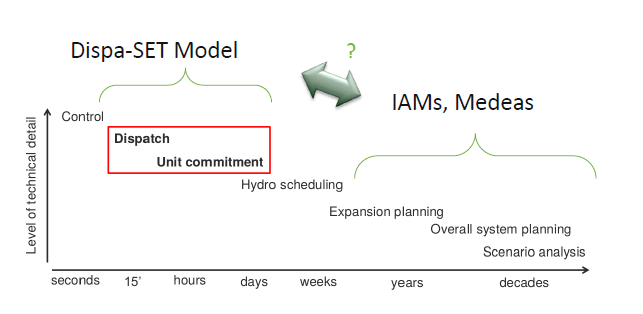
\includegraphics[width=0.8\textwidth]{resources/images/dispaset-medeas-timescale.png}
    \caption{An illustration of where Dispa-SET and MEDEAS operate on the timescale}
    \label{fig:dispaset-medeas-timescale}
\end{figure}

\subsubsection{Linking types}

There are several strategies that may be used in order to link two models together.

\begin{itemize}
    \item Soft linking: the models communicate between each other with feedback. Both of the models are run iteratively, thus keeping their separate efficiencies in the same order of magnitude. However, the iteration lead to low overall speed, and there is no guarantee of converging.
    \item Hard linking: the models are combined into a single, unified mathematical formulation. This newly created model can then be solved all at once. But this comes with a lower chance of computational feasibility.
\end{itemize}

These linking types are illustrated on Figure \ref{fig:linking-types}.

\begin{figure}[h]
    \centering
    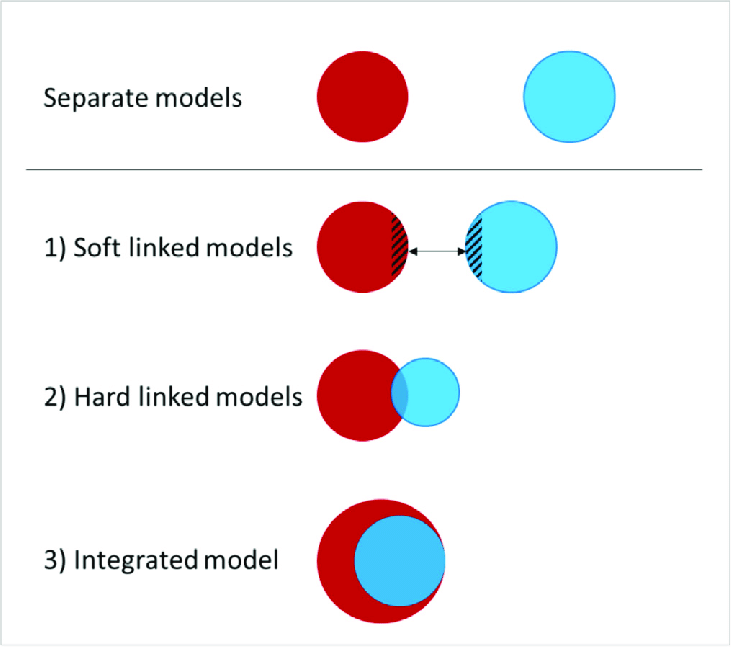
\includegraphics[width=0.4\textwidth]{resources/images/hybrid_model_variants.png}
    \caption{Illustration of the different linking methods \cite{hybrid_models}.}
    \label{fig:linking-types}
\end{figure}

One may also add model integration, consisting in completely embedding a model into the other. But this is not tractable in this setting, and would also requires compatible model formulations, as explained below.

In this case, hard linking is not possible due to the different formulations of Dispa-SET, in linear programming, and MEDEAS, in differential equations.

We also dismiss the soft linking strategy because of its slowness, and absence of convergence guarantee.

\subsubsection{Surrogate models}

As there are no good, viable linking options between Dispa-SET and MEDEAS, surrogate models are considered.

The idea behind surrogate models is simple. First, a fast, easy-to use approximation of the model is made, then it its completely integrated in the other model. In this case, the relevant outputs of the Dispa-SET model will be appriximated from relevant inputs regarding MEDEAS, then the approximator will be integrated in the model.

\subsection{State of the art in flexibility assessment}

As explained before, higher shares of VRES in the electricity production mix create the additional challenge, that is the handling of the partlially predictable variability of wind and sun energy. 

This handling requires a larger flexibility of the electrical system, that is, a better ability to adapt to changes in the demand and supply, either expected or not \cite{irena}.

To improve the flexibility of an existing power system, some mechanisms already exists.
\begin{itemize}
    \item Use of the regular dispatchable energy production plants to mitigate the energy not produced from VRES. Depending on the plant characteristics, it may be difficult to address short term drops in production, as there is some start up time required.
    \item Large interconnected electricity networks, that are able to smooth the VRES power output. There may be not enough sun in some region, creating a deficit, while there is too much in the neighboring country. By connecting them, the overproduction will compensate the unerproduction of the other.
    \item Energy storage facilities. Of course, storing the produced energy for later use is an easy way to account for the intermittency of the production. Typically, storing solar energy during day time to be used in the night. These technologies include pumped hydro-storage, batteries, compressed air. While pumped hydro-storage units are the most common, their very limited expansion options make them unlikely to grow in the future.
    \item Acting on the demand, in the extent that it can change its shape by promoting policies to the end users. Such policies focus on flattening the daily demand curve, facilitating the energy production dispatch. Typically, asking to delay greedy devices like dishwashers until night, where the overall demand is lower. But it may concern other domains, such as electric vehicles charge, heating and cooling etc.
\end{itemize}

The two main consequences of insufficiently flexible energy systems are curtailment, when there is too much energy produced, and load shedding, when there is not enough electricity to satisfy the demand. In case of load shedding, parts of the grid may be entirely shut down.

\subsection{This work}

\subsubsection{Objective}

This master's thesis is dedicated to the integration of the flexibility constraints, the Dispa-SET surrogate model, into the MEDEAS model, being less precise on the matter. This includes the creation of a proper dataset, the definition, training and integration of the surrogate model into MEDEAS.

\subsubsection{Methodology}

To do so, adequate design of experiment will be conducted on well-chosen input parameters, that will in fine be the surrogate model input features. This will give us a set of input points where a Dispa-SET run will be made, to create a training sample, and the samples are grouped into a single dataset.

Once this dataset is built, one can then train the surrogate model on it. This surrogate model is chosen after a short review of candidate machine learning options. It will be adequately fine tuned using hyper-parameter tuning.

When the model will be available, it will then be usable from inside MEDEAS, where some connection will have to be drawn between the variables that are already present in the model, and the surrogate model actual input and output features.

Finally, the resulting adapted MEDEAS model will be run, and observations and criticisms will be made.

\subsubsection{Contributions}

This works follows what was started by another student, Carla Vidal, that went until the surrogate model training, included. Given that improvements where implemented in Dispa-SET since then, the runs had to be re-done. However, there were no easy to use scripts to set up the simulation files etc., so that is has been chosen to write new ones.

Furthermore, the present thesis also considers other machine learning algorithms, although they are not actually implemented, the choice of neural networks is justified.

This work constisted in:
\begin{itemize}
    \item The writing of easy-to-use scripts to run Dispa-SET on those experiments
    \item The efinition and implementation of an adequate machine learning model (neural net), and training
    \item The integration the model in MEDEAS, by writing a C++ external function library for Vensim
    \item Runs and analysis of the improved MEDEAS model
\end{itemize}

All the produced work, and necessary data is available on the online github repository at the following address: \href{https://github.com/Rayerdyne/master-thesis}{https://github.com/Rayerdyne/master-thesis}\footnote{As it contains licensed file from Vensim, this repository is private. One may ask reading permission by email at \href{mailto:f.straet@student.uliege.be}{f.straet@student.uliege.be}.}

\subsubsection{Outline}

This document is structured as follows:

\begin{enumerate}
    \item \textbf{The Dispa-SET model}: description of the Dispa-SET model and tools
    \item \textbf{The MEDEAS model}: description of the MEDEAS model and framework
    \item \textbf{Data generation}: description of the complete process to generate the training data, that is, the design of experiments and the Dispa-SET runs
    \item \textbf{The surrogate model}: definition of the surrogate model, training and validation
    \item \textbf{Integration}: description of the process of integrating a model into MEDEAS
    \item \textbf{Analysis}: the analysis of the runs of MEDEAS with the integrated surrogate model
    \item \textbf{Conclusions}
\end{enumerate}
